\pdfminorversion=4
\pdfobjcompresslevel=1

\documentclass{beamer}
%\usetheme{Warsaw}
\usetheme{MAUA}
\setlength{\leftmargini}{20pt}

\usepackage[utf8]{inputenc}
\usepackage[T1]{fontenc}
\usepackage{minted}
\usepackage[brazil,brazilian]{babel}

\usepackage{tikz-timing}[2009/05/15]
\def\degr{${}^\circ$}

\usepackage{mdframed}
\definecolor{pearl}{rgb}{0.94, 0.92, 0.84}

\usepackage{graphicx}
\graphicspath{./Figs/}

\usepackage{todonotes}

\title{Processamento de Sinais}
\subtitle{HIL}
\author{Rafael Corsi Ferrão}
\date{\today}
\institute{\url{rafael.corsi@maua.br}}

\AtBeginSection[]
  {
     \begin{frame}<beamer>
     \frametitle{Conteúdo}
     \tableofcontents[currentsection]
     \end{frame}
}  

\begin{document}

\begin{frame}[plain,t]
	\titlepage
\end{frame}

\begin{frame}
	\frametitle{Conteúdo}
		\tableofcontents
\end{frame}

\section{HIL}

\subsection{Introdução}

\begin{frame}{HIL}{Hardware In-The-Loop}
	\begin{center}
	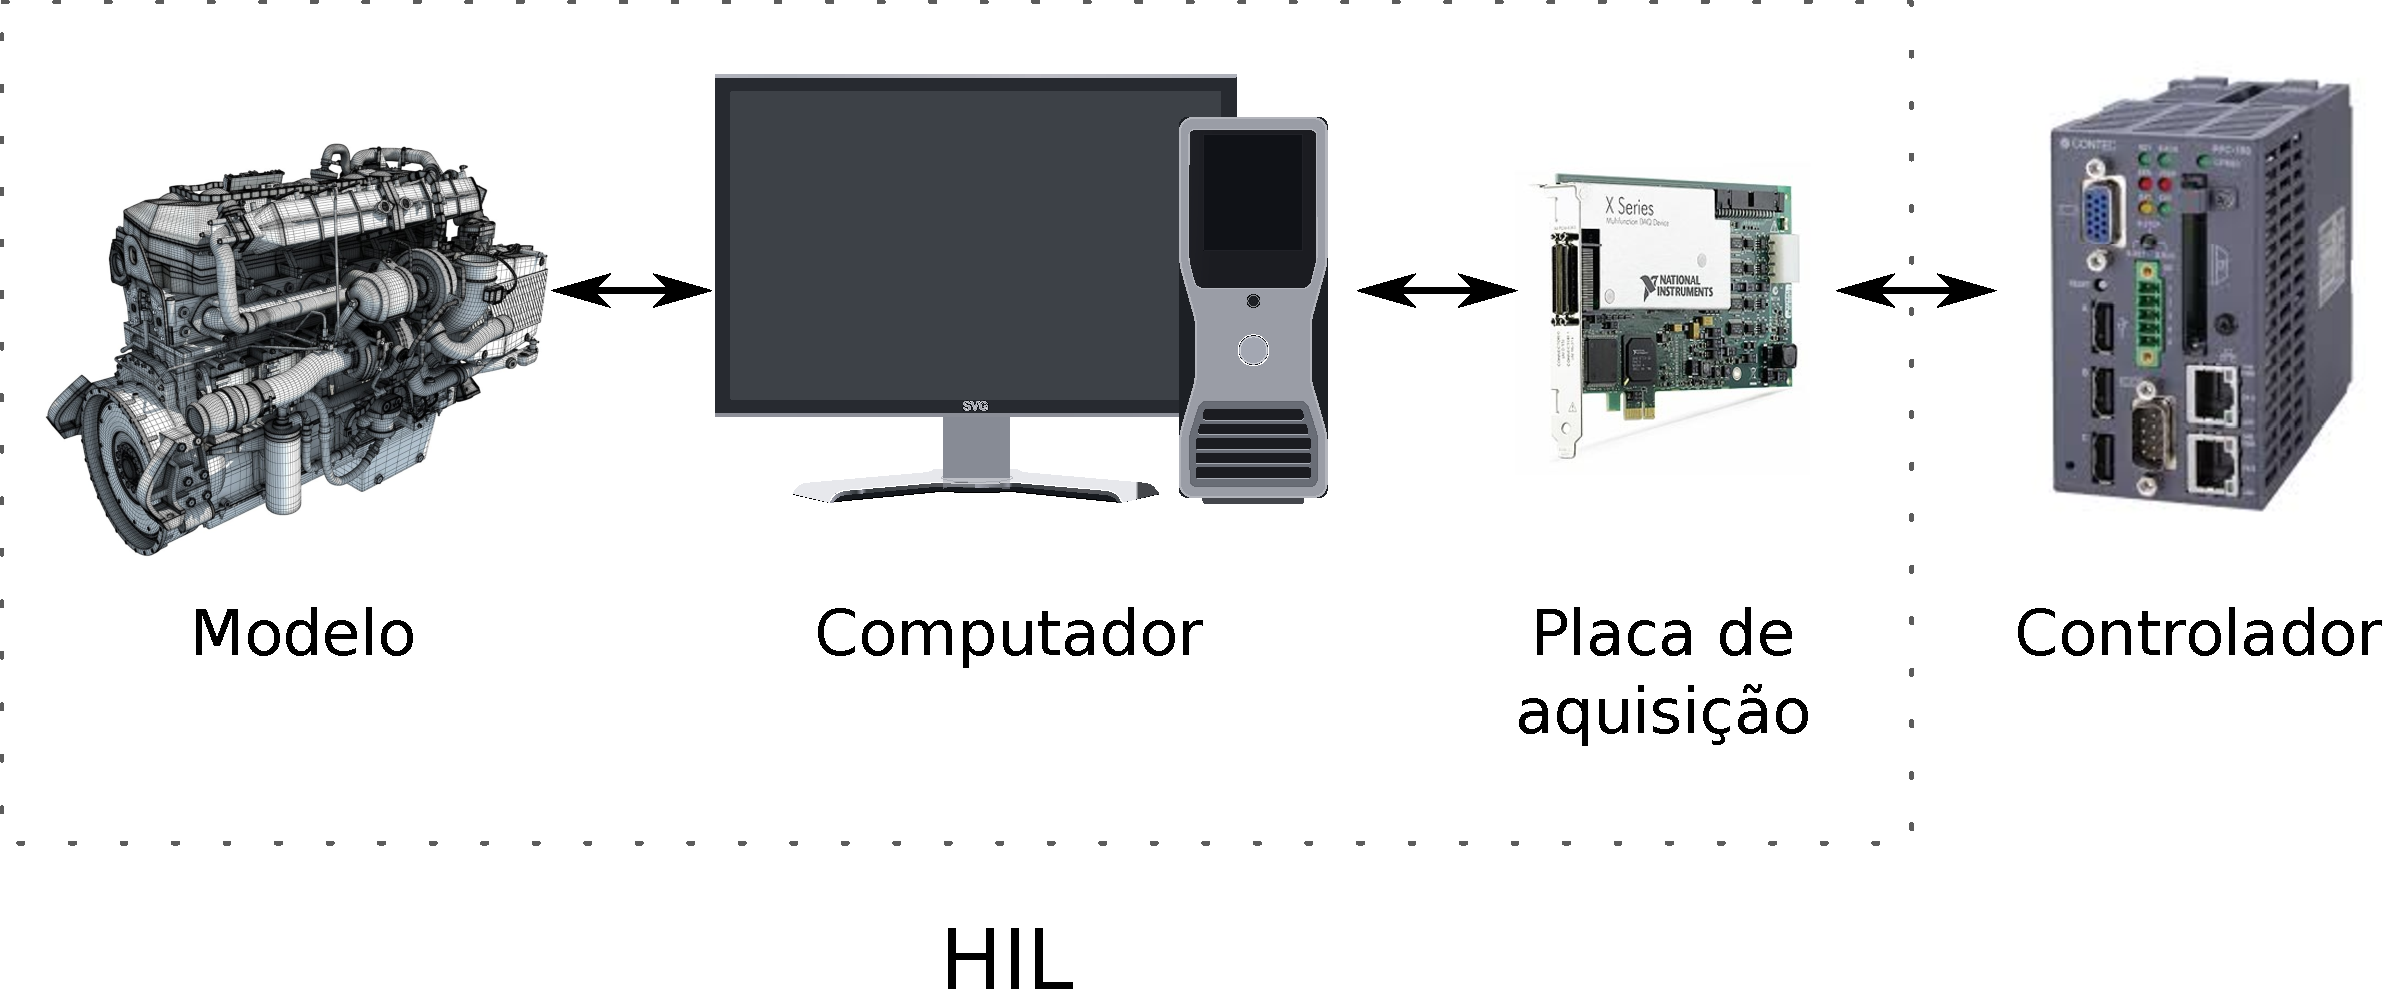
\includegraphics[width=0.9\linewidth]{hil}
	\end{center}
	
	\begin{itemize}
	\item Simulação HIL é uma técnica usada no desenvolvimento de sistemas complexos e críticos;
	\item a simulação HIL difere de uma simulação em tempo real (ex. simulink) por adicionar um sistema real ao loop.
	\end{itemize}
	
	A ideia é validar o controlador numa planta virtual antes de realizar testes reais.
\end{frame}

\begin{frame}{HIL}{Exemplo 1}
	\begin{center}
	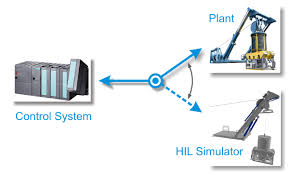
\includegraphics[width=0.8\linewidth]{hil3}
	\end{center}	
\end{frame}

\begin{frame}{Exemplo 1}
	\begin{center}
	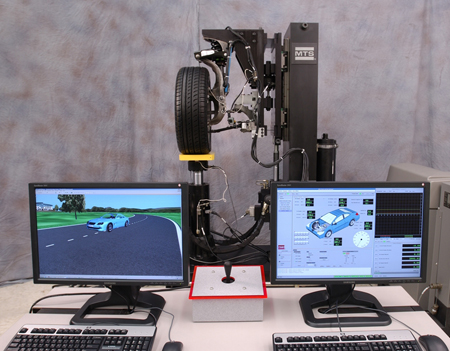
\includegraphics[width=0.9\linewidth]{hil_example}
	\end{center}
\end{frame}

\begin{frame}{HIL}{Porque usar ?}
	\begin{itemize}
		\item Aumenta a qualidade dos testes
		\item validação de sistemas críticos
		\item desenvolvimento mais rápido/barato
			\begin{itemize}
					\item otimiza as etapas no desenvolvimento em V
			\end{itemize}
	\end{itemize} 
	
	\begin{center}
	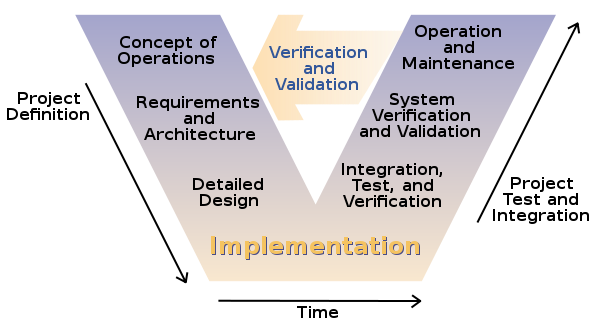
\includegraphics[width=0.8\linewidth]{vmodel}
	\end{center}	
\end{frame}

\begin{frame}{HIL}{Exemplos de aplicação}
	\begin{itemize}
		\item Planta nuclear
		\item Quadrirotor
		\item Satélite
		\item Sistemas médicos e hospitalares
		\item \ldots
	\end{itemize} 
\end{frame}

\subsection{Softwares}

\begin{frame}{HIL}{Softwares}
	Os principais SW de modelagens possuem suporte a HIL:
	
	\begin{itemize}
		\item Matlab/ Simulink
		\item LabView
	\end{itemize}	
	
	Para isso é preciso possuir uma placa de aquisição:
	
	\begin{center}
	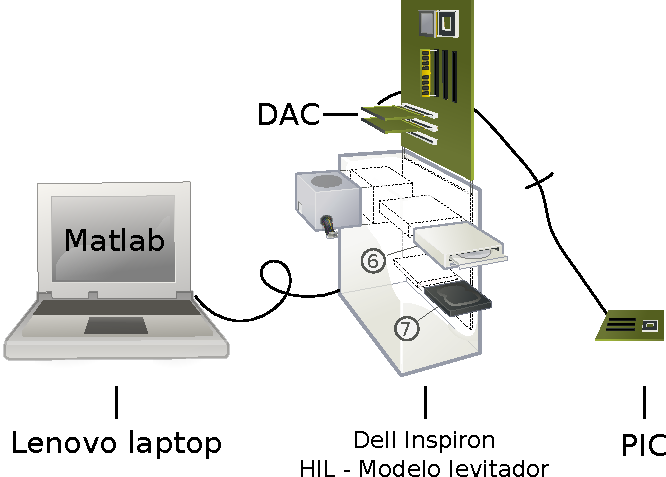
\includegraphics[width=0.5\linewidth]{material}
	\end{center}
\end{frame}

\begin{frame}{HIL}{Matlab}
	No Matlab, existem duas maneiras de realizar simulação HIL: 
	
	\begin{itemize}
	\item Simulink Desktop Real-Time :
	
	O computador com matlab é responsável por realizar os cálculos em tempo real e expor/ler os dados da placa de aquisição.
	
	\item Xpc Target:
	
	O sistema é compilado no Matlab e embarcado em um Hardware dedicado, a simulação é executada em modo Stand-alone.
	\end{itemize}

	\begin{center}
	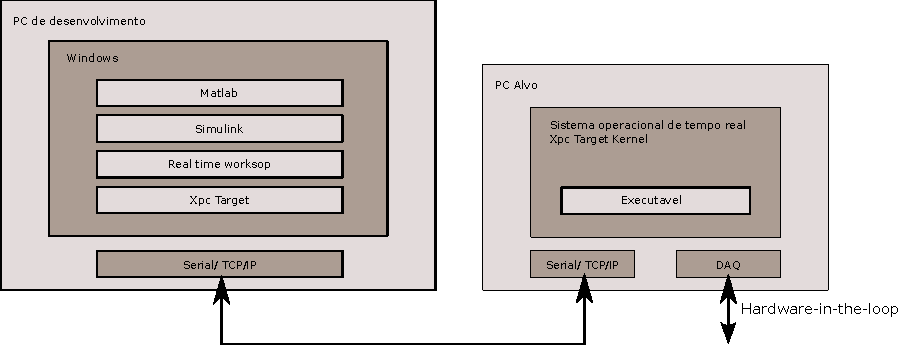
\includegraphics[width=0.8\linewidth]{flux-xpc}
	\end{center}
\end{frame}

\begin{frame}{DAQ}{Digital Aquisition Board}	
	Placa dedicada para aquisição de sinal, possui normalmente conversores A/D, D/A, saídas e entradas Digitais (PWM, Counter).
	
	A National Instruments é a principal fornecedor de placas de aquisição, o "Elvis" por exemplo utiliza o DAQ: PCI-6251 
	\footnote{\tiny \url{http://sine.ni.com/nips/cds/view/p/lang/pt/nid/14124}}
	
	\begin{center}
	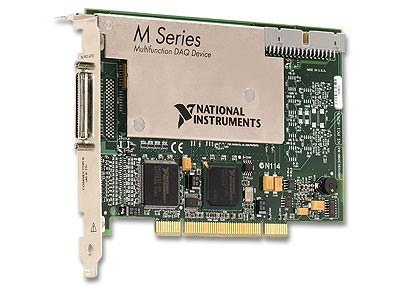
\includegraphics[width=0.4\linewidth]{pci_6251}
	\end{center}
\end{frame}

\subsection{Simulink}


\begin{frame}{Simulink}{Configuração}	

Simulação em External:

\begin{center}
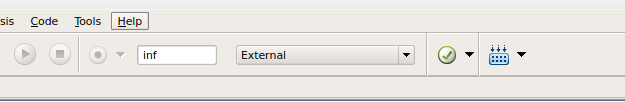
\includegraphics[width=0.7\linewidth]{simulink_config}
\end{center}

Passo de interação fixo, e configurado para a taxa de amostragem definida:

\begin{center}
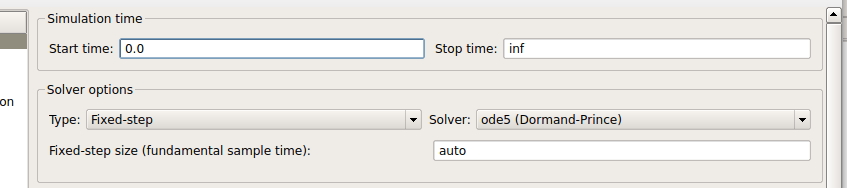
\includegraphics[width=0.7\linewidth]{simulink_config2}
\end{center}
\end{frame}

\begin{frame}{Simulink}{Configuração}	
	
	Escolha do modo de operação, nesse caso queremos que o PC com o matlab rode a simulação:

	\begin{center}
	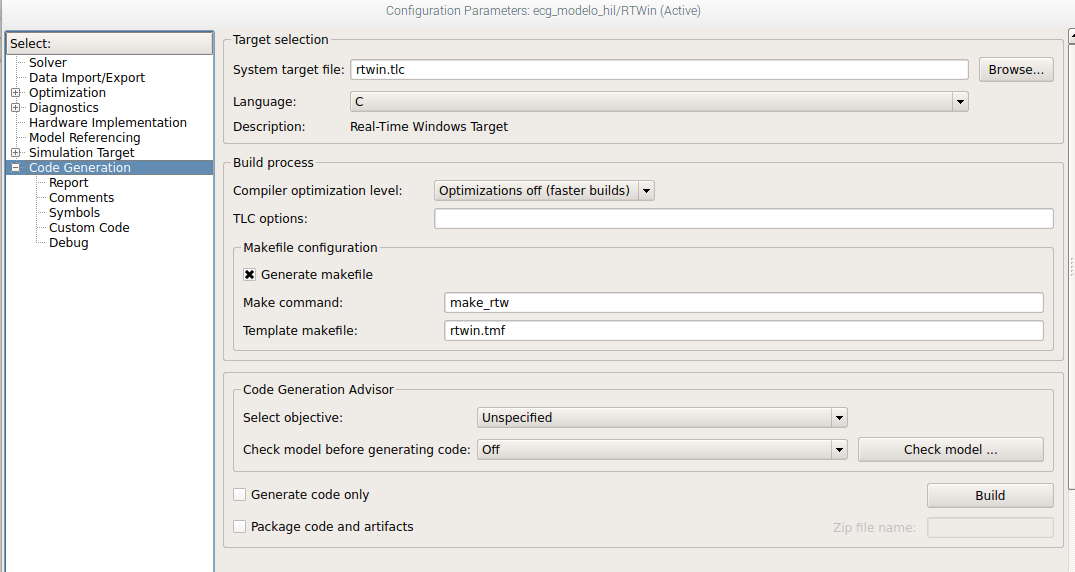
\includegraphics[width=1\linewidth]{simulink_config3}
	\end{center}
\end{frame}
% % % % % % % % % % % % % % %
\end{document}
% % % % % % % % % % % % % % %

